\chapter{GUI}

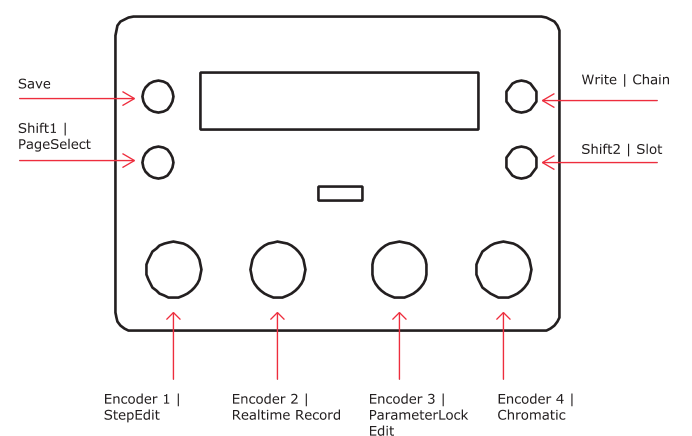
\includegraphics[scale=.6]{mcl_gui.png}\\

\section{Function Buttons:}
From the Grid Page, the MegaCommand's four upper function buttons are used to access the following Pages:
\begin{itemize}
\item{\textbf{[Save]}: Enters the Save page}
\item{\textbf{[Write | Chain]}: Enters the Write or Chain page}
\item{\textbf{[Shift1 | PageSelect]}: Opens the PageSelect menu}
\item{\textbf{[Shift2 | Slot]}: Opens the slot Menu }
\end{itemize}
Combined Button Presses:
\begin{itemize}
\item{\textbf{[Save] + [ Write | Chain ]}: Opens the Global Settings menu }
\end{itemize}
\\
\section{Encoder Buttons}
From the Grid Page the encoder buttons are used to access Sequencer Pages:
\begin{itemize}
\item{\textbf{[Encoder 1]}: Enter sequencer StepEdit page}
\item{\textbf{[Encoder 2]}: Enter sequencer RealTimeRecord page}
\item{\textbf{[Encoder 3]}: Enter sequencer ParameterLock page}
\item{\textbf{[Encoder 4]}: Enter sequencer Chromatic page}

\end{itemize}
\section{Trigger Interface}
Trigger Interface

\section{Global Settings}
Pressing Save + Write together will open the Global Settings page.

\section{Page Select}

\section{Sequencer Pages}
The 4 Encoder Buttons are used to enter the Ext Sequencer pages.

(Sub page indicated with [ ] brackets and activated with top right button)

Encoder 1: MD Step edit                         [ A4 Step edit ]
Encoder 2: MD Record Live                     [ MD Record Parameter Locks Live ]
Encoder 3: MD Parameter Lock Page A  [ MD Parameter Lock Page B ]
Encoder 4: MD/A4 Pitch Mode               [ MD/A4 Pitch Record Mod
